\documentclass{article}
\usepackage[utf8]{inputenc}

\usepackage{amsmath}
\usepackage{amsfonts}
\usepackage{accents}
\usepackage{graphicx}
\usepackage{geometry}
\usepackage{cancel}
 \geometry{
 a4paper,
 total={170mm,257mm},
 left=20mm,
 top=20mm,}

\newcommand{\rhocx}{(\rho c \Delta x)_f}

\title{\textbf{ME 511 Project 2}}

\author{\textbf{One Team}: \\ Obed Acevedo, Geoff Germino, Ramsey Ibrahim, Ryan Kelly, \\ Alex Pawlowski, Preetam Sharma, John Thress}

\date{October 8, 2019}


\begin{document}

\maketitle

\section{Introducing the Problem}

%%%%%%%%%%%%%%%%%%%%%%%%%%%%%%%%%%%%%%%%%%%%%%%%%%%%%%%%%%%%%

Show that

\begin{equation}
  \theta(0,t) = \frac{1}{(\rho c \Delta x)_f}\int_{u=0}^t q''_s(u)e^{\beta^2(t-u)/(\rho c \Delta x)^{2}_f} \ \text{erfc}\bigg(\frac{\beta}{(\rho c \Delta x)_f} \sqrt{t-u}\bigg)\text{d}u
    \label{thinfilm}
\end{equation}
reduces to

\begin{equation}
    \theta(0,t) = \frac{1}{\beta\sqrt{\pi}}\int_{u=0}^t\frac{q''_s(u)}{\sqrt{t-u}}\text{d}u, \   t\geq 0, \   \text{as} \   \Delta x \xrightarrow{}0.
    \label{reduced}
\end{equation}
\newline 
Here, $\theta=T-T_0$, where $\theta$ is called the reduced temperature. The property grouping $\rho c \Delta x$ is associated with a thin film $f$ located on the surface of a semi-infinite substrate. The thickness of the film is $\Delta x$. The thermal product is denoted as $\beta$ and is $\sqrt{\rho c k}$ of the substrate. Here, $t$ is time and $u$ is a dummy variable of time.
\newline
\newline
\noindent(\emph{Hint:} Let $ z=\frac{\beta\sqrt{t-u}}{(\rho c \Delta x)_f} \geq 0 $.                                    Notice that $z\rightarrow\infty$  as $ \Delta x\rightarrow 0 $ for $ u \ne t$.)

\subsection*{Significance}
This reduction is important as the original Eq. \eqref{thinfilm} suggests a discontinuity of the reduced temperature as the thin film is reduced to 0, when it should otherwise return the heat equation, as the reduced equation \eqref{reduced} shows.
%%%%%%%%%%%%%%%%%%%%%%%%%%%%%%%%%%%%%%%%%%%%%%%%%%%%%%%%%%%%%

\section{Recall}

\subsection*{L'Hôpital's Rule}
When finding the limit of the division of 2 functions, one may encounter an indeterminate form
\begin{equation*}
    \mathop {\lim }\limits_{x \to a} \frac{{f\left( x \right)}}{{g\left( x \right)}} = \frac{0}{0}\hspace{0.25in}{\mbox{OR}}\hspace{0.25in}\mathop {\lim }\limits_{x \to a} \frac{{f\left( x \right)}}{{g\left( x \right)}} = \frac{{ \pm \,\infty }}{{ \pm \,\infty }}
\end{equation*}
In calculus, L'Hôpital's Rule can be used to rectify the above indeterminate forms, provided the differentials can be found, with the below substitution:
\begin{equation*}
    \mathop {\lim }\limits_{x \to a} \frac{{f\left( x \right)}}{{g\left( x \right)}} = \mathop {\lim }\limits_{x \to a} \frac{{f'\left( x \right)}}{{g'\left( x \right)}}
\end{equation*}

\section{Solution}

Using the hint given, two additional expressions can be obtained by taking the square of $ z $ and the reciprocal of $(\rho c \Delta x)_f$:

\begin{equation}
    z^2=\frac{\beta^2(t-u)}{(\rho c \Delta x)^2_f}
\end{equation}
and
\begin{equation}
    \frac{1}{(\rho c \Delta x)_f}=\frac{z}{\beta\sqrt{{t-u}}}
\end{equation}
The constant term $\frac{1}{(\rho c \Delta x)_f}$ is absorbed into the integral so that the expression 

\begin{equation}
  \theta(0,t) =\int_{u=0}^t\frac{q''_s(u)e^{\beta^{2(t-u)}/(\rho c \Delta x)^{2}_f}}{(\rho c \Delta x)_f} \text{erfc}\bigg(\frac{\beta}{(\rho c \Delta x)_f} \sqrt{t-u}\bigg)\text{d}u
\end{equation}
is obtained. The new expressions can be plugged into the original equation  \eqref{thinfilm} so that now one has
\begin{equation}
   \theta(0,t)=\int_{u=0}^t\frac{q''_s(u)}{\beta\sqrt{t-u}}ze^{z^2}\text{erfc}(z)\text{d}u.
\end{equation}
By taking the limit $z \rightarrow \infty$, one obtains the expression

\begin{equation}
    \lim_{z\rightarrow\infty} \theta(0,t) = \lim_{z\rightarrow\infty} \int_{u=o}^t \frac{q''_s(u)}{\beta\sqrt{t-u}} ze^{z^2} \text{erfc}(z)\text{d}u.
    \label{taketolimit}
\end{equation}

\newline 
The simplification of this expression will come from being able to bring the limit inside the integrand. To do so, one needs to show that the limit $z \rightarrow \infty$ exists of the integrand. % Where is this step?
Defining $f_z \equiv ze^{z^2} \text{erfc}(z)$, the limit takes the form
% Let $ze^{z^2} \text{erfc}(z)$ be equal to $f_z$ // I changed this to the above form

\begin{equation}
        \lim_{z\rightarrow\infty} \int_{u=o}^t \frac{q''_s(u)}{\beta\sqrt{t-u}} f_z \text{d}u.
\end{equation}
When the limit of $f_z$ is evaluated, an indeterminate result is obtained:

\begin{equation}
    \lim_{z\rightarrow\infty}f_z = \lim_{z\rightarrow\infty}[ ze^{z^2} \text{erfc}(z)] = \infty \cdot 0.
\end{equation}
To solve this, the expression must be written in such a way that either $\frac{0}{0} $ or $\frac{\infty}{\infty} $ are obtained in order to apply L’Hôpital’s rule which would solve the limit. By changing the expression to 

\begin{equation}
    \lim_{z\rightarrow\infty}\frac{ \text{erfc}(z)}{ (ze^{z^2})^{-1}},
\end{equation}
the limit is effectively expressed as $\frac{0}{0} $. This is because as the error function values go to infinity, the value becomes zero:

\begin{figure}[h]
    \centering
    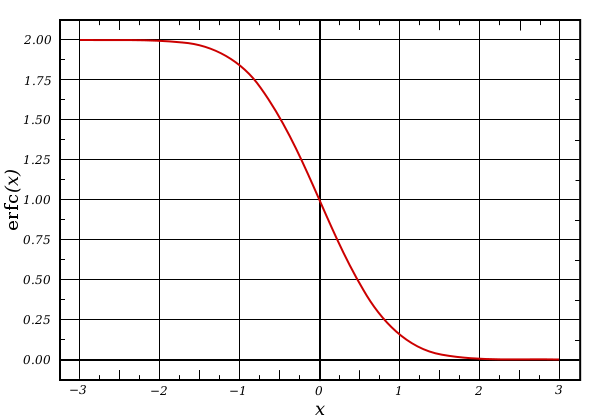
\includegraphics[width=9cm\textwidth]{erfcplot}
    \caption{erfc function plot}
    \label{erfcplot}
\end{figure}

\noindent L’Hôpital’s rule can now be applied:

\begin{equation}
     \lim_{z\rightarrow\infty}\frac{ \text{erfc}(z)}{ (ze^{z^2})^{-1}} =  \lim_{z\rightarrow\infty}\frac{\frac{d}{dz}\text{erfc}(z)}{\frac{d}{dz}(ze^{z^2})^{-1}}.
\end{equation}
Both derivatives are now evaluated. By definition:

\begin{equation}
    \frac{d}{dz}(\text{erfc}(z)) = \frac{d}{dz} \bigg(1-\frac{2}{\sqrt{\pi}}\int_{0}^{z} e^{-\alpha^2}\text{d}\alpha\bigg).
\end{equation}
Evaluating the first derivative yields

\begin{equation}
    \frac{d}{dz} \bigg(1-\frac{2}{\sqrt{\pi}}\int_{0}^{z} e^{-\alpha^2}\text{d}\alpha\bigg) = \frac{-2}{\sqrt{\pi}}\frac{d}{dz}\bigg(\int_{0}^{z} e^{-\alpha^2}\text{d}\alpha\bigg) = -\frac{2e^{-z^2}}{\sqrt{\pi}},
\end{equation}
and evaluating the second derivative yields

\begin{equation}
    \frac{d}{dz}\bigg(\frac{e^{-z^2}}{z}\bigg) = \frac{d}{dz}(z^{-1}e^{-z^2})=(2z)+z^{-2}e^{-z^2}(-1) = -2e^{-z^2} - \frac{e^{-z^2}}{z^2}.
\end{equation}
Now the result can be expressed as 

\begin{equation}
    \lim_{z\rightarrow\infty}\frac{ \text{erfc}(z)}{\bigg(\frac{e^{-z^2}}{z}\bigg)} =  \lim_{z\rightarrow\infty}\frac{\frac{-2}{\sqrt{\pi}}e^{-z^2}}{-2e^{-z^2} - \frac{e^{-z^2}}{z^2}} = \lim_{z\rightarrow\infty} \frac{\frac{1}{\sqrt{\pi}}}{1-\frac{\frac{e^{-z^2}}{z^2}}{-2e^{-z^2}}}=\lim_{z\rightarrow\infty} \frac{\frac{1}{\sqrt{\pi}}}{1+\frac{2}{z^2}}.
\end{equation}
Taking this limit now yields

\begin{equation}
 \lim_{z\rightarrow\infty} [ze^{z^2}\text{erfc}(z)]
 = \lim_{z\rightarrow\infty} \frac{\frac{1}{\sqrt{\pi}}}{1+\frac{2}{z^2}}  
 = \frac{1}{\sqrt{\pi}}
 \label{limiteval}
\end{equation}
As the limit exists for $ze^{z^2}$ as $z \rightarrow \infty$, the limit can be rearranged inside the integrand. Because the heat flux term is constant with respect to $z$, it can be moved outside of the limit. Eq. \eqref{taketolimit} can now be rearranged to

\begin{equation}
    \lim_{z\rightarrow\infty} \theta(0,t) = \int_{u=o}^t \frac{q''_s(u)}{\beta\sqrt{t-u}} \lim_{z\rightarrow\infty}[ ze^{z^2} \text{erfc}(z)]\text{d}u.
\end{equation}
By substituting the limit \eqref{limiteval} back into the expression, the expression reduces to

\begin{align}
    \theta(0,t) &= \frac{1}{\beta}\int_{u=0}^t \frac{q''_s(u)}{\sqrt{t-u}}\bigg(\frac{1}{\sqrt{\pi}}\bigg)\text{d}u \\
     \theta(0,t) &= \frac{1}{\beta\sqrt{\pi}}\int_{u=0}^t\frac{q''_s(u)}{\sqrt{t-u}}\text{d}u \hspace{0.25in} \text{When } t  \geq 0 \text{ as } \Delta x \rightarrow 0
\end{align}

%%%%%%%%%%%%%%%%%%%%%%%%%%%%%%%%%%%%%%%%%%%%%%%%%%%%%%%%%%%%%

\section{Conclusion}

Using substitution and L'Hôpital's Rule, one can find that the original expression \eqref{thinfilm} for the reduced temperature through a thin film on the surface of a semi-infinite substrate still satisfies the heat equation as the film thickness approaches 0.
%%%%%%%%%%%%%%%%%%%%%%%%%%%%%%%%%%%%%%%%%%%%%%%%%%%%%%%%%%%%%

\end{document}
